%!TEX program = xelatex
% chktex-file 2
% chktex-file 8
% chktex-file 12
% chktex-file 13
% chktex-file 24
% chktex-file 36
% chktex-file 44
\documentclass[12pt]{article}

\usepackage[english]{babel}
\usepackage{xeCJK}

% Set page size and margins
\usepackage[a4paper,top=2cm,bottom=2cm,left=3cm,right=3cm,marginparwidth=1.75cm]{geometry}

% Useful packages
\usepackage{amsmath}
\usepackage{graphicx}
\usepackage[colorlinks=true, allcolors=blue]{hyperref}
\usepackage{xurl}

\usepackage{array}
\newcolumntype{P}[1]{>{\centering\arraybackslash}p{#1}}
\newcolumntype{M}[1]{>{\centering\arraybackslash}m{#1}}

\usepackage{adjustbox}
\usepackage{caption}
\usepackage{subcaption}
\usepackage{siunitx}
\usepackage{float}
\usepackage{booktabs}
\usepackage{tabularx}
\usepackage{multirow}
\usepackage{setspace}
\usepackage{fbox}

% ----- paragraph -----
\usepackage{titlesec}
\setcounter{secnumdepth}{4}
\titleformat{\paragraph}
{\normalfont\normalsize\bfseries}{\theparagraph}{1em}{}
\titlespacing*{\paragraph}
{0pt}{3.25ex plus 1ex minus .2ex}{1.5ex plus .2ex}
% ----- paragraph ----

\setCJKmainfont{NotoSerifTC-Regular}[
  AutoFakeBold = 3
]
\setCJKmonofont{NotoSerifTC-Regular}

\usepackage{indentfirst}
\setlength\parindent{24pt}
\setlength{\parskip}{0.35em}
\setstretch{1.08}

% placeholder box for missing figures
\newcommand{\figplaceholder}[2]{%
  \fbox{\parbox{\dimexpr#1-2\fboxsep-2\fboxrule\relax}{%
    \centering\vspace{1.5cm}【圖片待補：#2】\vspace{1.5cm}%
  }}%
}

\begin{document}

\begin{titlepage}
  \begin{center}
      \vspace*{1cm}
       \begin{LARGE}
           \textbf{
           \\數位電子學實務
           }
       \end{LARGE}

       \begin{LARGE}
            \textbf{
            \\ -- 期末書面結案報告 --
        }
        \end{LARGE}

      \vspace{1cm}
        \textbf{抬底仔(á)-Tidy UP}

      \vspace{1.5cm}

      \textbf{Group 2: B11702091 張容爾, B10901144 王俊皓}

      \vspace{1.5cm}

      \text{\today}

      \vspace{0.8cm}

      
\includegraphics[width=0.7\textwidth]{figure/car.png}

      \vfill

      \vspace{0.8cm}

  \end{center}
\end{titlepage}

% ---------------------------------------------------------------
\section{專題基本介紹}
% ---------------------------------------------------------------

\subsection{研究背景與動機 (Why)}

根據國家衛生研究院高齡醫學暨健康福祉研究中心在《臺灣高齡健康與長照服務年報》之統計，台灣由高齡者組成之家戶數逐年攀升，其中獨居長者家戶亦呈現持續成長（國家衛生研究院高齡醫學暨健康福祉研究中心，n.d.），加上台灣已於 2025 年正式邁入超高齡社會，65 歲以上人口占比突破 20\%，高齡生活的安全議題已不容忽視。在眾多高齡風險中，「跌倒」對長者的威脅尤為顯著，依衛生福利部統計處公布之 107 年國人死因統計結果，跌倒高居 65 歲以上長者事故傷害死亡原因第二位（每十萬人 25.7 人）（衛生福利部統計處，2021）。此外，衛生福利部新聞稿並援引國民健康署 106 年「國民健康訪問調查」指出，65 歲以上長者每 6 人就有 1 人在過去一年內曾經跌倒（15.5\%）（衛生福利部，2019）。

值得注意的是，跌倒的成因與居家環境高度相關。國民健康署指出，長者跌倒危險因子可分為社會人口學因子、身心功能與疾病用藥因子，以及環境因子三大類，其中居家環境之照明不足、地板髒亂、地毯未固定與走道堆放雜物等，皆為常見潛在危害（衛生福利部國民健康署，n.d.）。由此可知，長者跌倒不只是「多發生在家中」，家中環境本身的失序更是致跌的關鍵推手。日常生活中，散落的拖鞋、未收好的電線等小型障礙物看似不起眼，卻經常是絆倒長者的主因。對此，國民健康署提出「規律運動、維持居家環境、用藥安全」三大防跌原則（衛生福利部，2019），本組的提案選擇從「維持居家環境」切入，期望透過排除家中常見的地面風險，降低長者因跌倒而受傷的機率。

\subsection{執行方法評估 (How)}

為達成「維持居家環境」的目標，讓長者能安全地在家中走動，我們評估了教育宣導、行為監控、居住環境改造等多種可能路徑，最終選擇以「單一遠端操控拾物裝置」來直接改善居家地面環境，期望能以最低的能耗與空間佔用，讓環境在人機協作下維持安全狀態，同時保留長者最大的活動自由。

\subsubsection{解決方案比較}

以下為我們評估過的四類方案與取捨理由，並附各方案估計兩年成本以供比較：

\begin{itemize}
  \setlength{\itemsep}{0.5em}
  \item \textbf{教育宣導、改變長者行為（兩年估計 19 萬元）：} 透過環境改造所達到的防跌效果往往優於僅依賴行為提醒（Pynoos et al., 2010），單純宣導難以長期落實，故效果有限。
  \item \textbf{偵測通報系統（兩年估計 16.3 萬元）：} 如監視器透過影像偵測跌倒，或智慧手錶監測身體訊號。此類方法雖能即時發現意外，但影像式跌倒偵測的主要挑戰之一為隱私侵犯（Wang et al., 2020），容易引發長者疑慮，且無法從根本解決跌倒風險。
  \item \textbf{居家照護、聘請專業看護（兩年估計 28.2 萬元）：} 此為目前最常見且有效的方案，但受限於照護人力短缺與成本攀升，長照費用對家庭造成顯著負擔（TIME, 2025），故難以作為普遍可行的解法。
  \item \textbf{抬底仔 (á)-Tidy UP（兩年成本不到 1 萬元）：} 以遠端操控方式主動撿拾居家地面障礙物，具備成本效益佳、全天候守護、無侵入感、操控直覺等優勢，為本組所選擇之方案。
\end{itemize}

\subsubsection{本專案設計目標}

確立方向後，我們為\textbf{抬底仔 (á)-Tidy UP} 訂定三項核心設計目標：

\begin{enumerate}
  \setlength{\itemsep}{0.3em}
  \item 具備基本避障能力，在室內環境中安全移動。
  \item 低成本、低能耗、低隱私疑慮，且具備可擴充性。
  \item 降低對長者主動整理環境的依賴。
\end{enumerate}

\subsubsection{系統架構}

本系統設計源自 Cook 與 Das 所提出的智慧環境系統架構（Cook \& Das, 2004），以「感知—決策—執行」的循環維持居家環境地面秩序，如表 \ref{tab:architecture} 所示。

\begin{table}[H]
  \centering
  \caption{感知—決策—執行系統架構}
  \label{tab:architecture}
  \renewcommand{\arraystretch}{1.4}
  \begin{tabularx}{\textwidth}{c X X}
    \toprule
    \textbf{階段} & \textbf{核心元件} & \textbf{功能說明} \\
    \midrule
    感知 & ESP32、HC SR-04 超聲波感測器、SG90 伺服馬達 & 驅動感測器左右掃描，量測各角度障礙物距離 \\
    決策 & Raspberry Pi 5 + Arduino UNO & 整合感測訊號，進行目標判定並透過網頁介面接收遠端指令 \\
    執行 & 步進馬達四輪底盤、多軸機械手臂 & 靠近目標物、以手爪夾取並送回指定位置 \\
    \bottomrule
  \end{tabularx}
\end{table}

% ---------------------------------------------------------------
\section{執行過程說明}
% ---------------------------------------------------------------

\subsection{所需元件與成本評估}

\subsubsection{所需元件}

我們參考市售避障車設計（CGTrader, n.d.）與多軸機械手臂相關之 DIY 實作（Instructables, n.d.-a, n.d.-b），依最終實作選擇列出各模組所需元件，如表 \ref{tab:materials} 所示。

\begin{table}[H]
    \centering
    \caption{最終零件清單}
    \label{tab:materials}
    \scriptsize
    \setlength{\tabcolsep}{3pt}
    \renewcommand{\arraystretch}{0.95}
    \begin{tabularx}{\linewidth}{l X X}
      \toprule
      車體功能 & 項目 & 用途 \\
      \midrule
      \multirow{3}{*}{感測避障}
        & ESP32 微控制器              & 左右掃描、障礙物距離量測與無線通訊 \\
        & HC SR-04 超聲波感測器       & 透過聲波反射量測前方距離（20--400 cm）\\
        & SG90 伺服馬達               & 驅動感測器進行 180° 左右掃描 \\
      \midrule
      \multirow{2}{*}{通訊/控制}
        & Raspberry Pi 5            & 主控電腦，負責網頁伺服器架設與高階決策 \\
        & Arduino UNO               & 負責底層馬達驅動訊號控制 \\
      \midrule
      \multirow{4}{*}{車身構造}
        & A4988 步進馬達驅動版         & 提供步進馬達精準電流控制 \\
        & A4988 模組                  & 控制步進馬達方向與步數 \\
        & 步進馬達                    & 驅動四輪底盤，提供可重複精準定位 \\
        & 車身結構                    & 承載所有元件之底盤框架 \\
      \midrule
      \multirow{3}{*}{機械手臂}
        & MG996R 伺服馬達             & 控制手臂大關節之旋轉與升降 \\
        & SG90 伺服馬達               & 控制手爪開合夾取動作 \\
        & 機身結構                    & 手臂本體支撐件與各關節連接件 \\
      \midrule
      \multirow{3}{*}{能量來源}
        & 12V 鋰電池 + AA 電池        & 提供底盤與機械手臂之驅動電力 \\
        & 12V 轉 5V 降壓變壓器        & 為控制板獨立提供穩定 5V 電源 \\
        & 保險系統                    & 過電流保護，防止短路損壞元件 \\
    \bottomrule
    \end{tabularx}
  \end{table}

\subsubsection{成本評估}

\begin{table}[H]
  \centering
  \caption{最終成本評估表}
  \label{tab:costs}
  \scriptsize
  \setlength{\tabcolsep}{3pt}
  \renewcommand{\arraystretch}{0.95}
  \begin{tabularx}{\linewidth}{l X r c r}
    \toprule
    車體功能 & 項目 & 單價（\$） & 數量 & 小計（\$）\\
    \midrule
    \multirow{3}{*}{感測避障}
      & ESP32 微控制器               & 185   & 1 & 185 \\
      & SG90 伺服馬達（感測用）        & 32    & 1 & 32 \\
      & HC SR-04 超聲波感測器         & 60    & 1 & 60 \\
    \midrule
    \multirow{2}{*}{通訊/控制}
      & Raspberry Pi 5              & 6{,}000 & 1 & 6{,}000 \\
      & Arduino UNO                 & 140   & 1 & 140 \\
    \midrule
    \multirow{4}{*}{車身構造}
      & A4988 步進馬達驅動版           & 180   & 1 & 180 \\
      & A4988 模組                   & 120   & 1 & 120 \\
      & 步進馬達                     & 600   & 1 & 600 \\
      & 車身結構                     & 200   & 1 & 200 \\
    \midrule
    \multirow{3}{*}{機械手臂}
      & MG996R 伺服馬達              & 360   & 1 & 360 \\
      & SG90 伺服馬達（手爪用）        & 180   & 1 & 180 \\
      & 機身結構                     & 200   & 1 & 200 \\
    \midrule
    \multirow{3}{*}{能量來源}
      & 12V 鋰電池 + AA 電池         & 280   & 1 & 280 \\
      & 12V 轉 5V 降壓變壓器         & 140   & 1 & 140 \\
      & 保險系統                     & 100   & 1 & 100 \\
    \midrule
    \multicolumn{4}{r}{\textbf{實際總計}} & \textbf{\$ 8{,}777}\\
    \bottomrule
  \end{tabularx}
  \par\vspace{4pt}
  \begin{flushleft}
    \footnotesize 註：價格查詢自蝦皮賣家、傑森創工、祥昌電子等網路商城。
  \end{flushleft}
\end{table}

\subsection{成員分工}

兩人均共同參與提案發想與時程規劃。細部分工上，張容爾獨力負責車體結構設計、機械手臂製作與元件配置，並協同參與車體電路與硬體程式的實作；王俊皓則主導感測避障系統的軟硬體整合、Raspberry Pi 網頁伺服器架設與 Arduino 底層控制程式撰寫。

\subsection{預期執行時程}

為確保\textbf{抬底仔(á)-Tidy UP}能如期完成，於提案階段我們依功能模組制定了以下週進度目標，如表 \ref{tab:schedule} 所示。

\begin{table}[H]
    \centering
    \caption{提案階段預期每週執行時程}
    \label{tab:schedule}
    \renewcommand{\arraystretch}{1.4}
    \begin{tabularx}{\textwidth}{c |l| X}
        \toprule
        \textbf{預定日期} & \textbf{階段性目標} & \textbf{預期成果與具體執行項目} \\
        \midrule
        04/24 & 基礎載具建置 & 完成基礎避障車之硬體組裝，確認車體移動與馬達控制功能正常。 \\
        05/01 & 感測器之整合 & 裝設超聲波感測模組，完成近距離障礙物偵測與基礎避障測試。 \\
        05/08 & 進階環境探測 & 導入光學雷達系統進行環境掃描，提升障礙物偵測精準度。 \\
        05/15 & 回收機構實作 & 完成拾物機構初步設計與組裝，使機器人具備接觸目標物的能力。 \\
        05/22 & 機構動作優化 & 改良拾物機構動作流暢度與穩定性，確保物品能被確實回收。 \\
        05/29 & 原型機展示 & 軟硬體系統整合完畢，進行初步可運行成品之進度報告與 Demo。 \\
        06/05 & 細部優化改良 & 針對測試反饋進行除錯、軟體參數調整與硬體細部改良。 \\
        06/12 & 期末完整驗收 & 繳交期末報告，展示具備自主探測與物品回收能力之拾物機器人。 \\
        \bottomrule
    \end{tabularx}
\end{table}

\subsection{預期與實際執行之差異}

實際開發過程中，因技術可行性與整合複雜度，各模組均有不同程度的調整，以下彙整五項主要差異：

\begin{enumerate}
  \setlength{\itemsep}{0.6em}

  \item \textbf{控制架構：由單一 Arduino 擴展為 Arduino + Raspberry Pi 雙控架構}

  提案階段規劃以 Arduino UNO R4 WiFi 作為唯一主控，整合通訊與馬達控制。實作中發現，若要同時支援 YOLO 物件辨識與即時遠端控制，Arduino 的運算能力嚴重不足，因此導入 Raspberry Pi 5 負責高階處理與網頁伺服器，Arduino UNO 則專責底層訊號控制，形成前後端分工的雙控架構。

  \item \textbf{感測模組：由人體紅外線感測器改為超聲波感測器搭配 ESP32}

  原規劃以 HC-SR501 人體紅外線感測器（PIR）進行避障偵測，但 PIR 僅能偵測發熱物體，無法有效感知拖鞋等常溫障礙物。因此改採 HC-SR04 超聲波感測器結合 ESP32 進行距離量測，搭配 SG90 伺服馬達進行 180° 左右掃描，大幅提升障礙物偵測的通用性與精準度。

  \item \textbf{驅動系統：由直流馬達改為步進馬達}

  原提案選用 L298N 馬達驅動板配合 DC 馬達，因其調速靈活且成本較低。但 DC 馬達在低速運行時容易因摩擦力變化導致位置漂移，影響拾物精準度。最終改用 A4988 步進馬達驅動板搭配步進馬達，以固定步數控制車輪旋轉角度，提高底盤移動的可重複性。

  \item \textbf{拾物機構：由鏟手改為多軸機械手臂}

  原設計以鏟片與畚箕作為主要拾物機構，透過伺服馬達驅動鏟片下降後鏟起目標物。實作測試中發現，鏟手在不平整地面上容易卡住，且無法夾取高度較高的物品。因此改採多軸機械手臂設計，以 MG996R 伺服馬達控制大關節旋轉，SG90 伺服馬達控制手爪，顯著提升拾物的適應性與成功率。

  \item \textbf{自主程度：由全自主 AI 辨識改為人機協同遠端遙控}

  提案階段規劃導入 YOLO 即時物件辨識，使機器人能自主判斷目標物位置並規劃路徑（Redmon et al., 2016）。由於 YOLO 模型在嵌入式硬體上的推論速度與準確度難以兼顧，且訓練資料集建立需要大量時間，最終調整為人機協同的遠端遙控模式，由操作者透過網頁介面即時判斷目標並下達控制指令，機器人負責精確執行移動與夾取。

\end{enumerate}

\subsection{關鍵困難與解決策略}

\begin{enumerate}
  \setlength{\itemsep}{0.6em}

  \item \textbf{多元件共用電源造成控制板重置}

  Raspberry Pi、Arduino、步進馬達與伺服馬達共用電源時，馬達驅動瞬間電流過大導致控制板重置。解決策略為將 12V 鋰電池透過降壓模組為控制板獨立供電，並加入保險絲保護電路，穩定整體供電架構。

  \item \textbf{機械手臂夾取穩定性不足}

  初版手臂設計夾取角度固定，遇到不同形狀的物品時成功率偏低。透過調整 SG90 伺服馬達的 PWM 訊號範圍與手爪開合角度，並在夾爪加裝防滑墊，改善夾取穩定度。

  \item \textbf{無線通訊延遲影響操控體驗}

  Raspberry Pi 架設之網頁控制介面初版在區域網路下存在約 300ms 的控制延遲，導致操作有明顯落差。透過優化網頁前端的事件監聽機制與後端 WebSocket 通訊協定，將延遲降低至可接受範圍，提升操控即時性。

\end{enumerate}

% ---------------------------------------------------------------
\section{成果分析}
% ---------------------------------------------------------------

\subsection{車體構造}

經歷提案階段之 3D 建模規劃（圖 \ref{fig:actual_robot}）與實際組裝，最終成品如圖 \ref{fig:actual_robot} 所示。車體以步進馬達四輪底盤為主體，多軸機械手臂安裝於前端，ESP32 感測模組置於車頂，Raspberry Pi 5 與 Arduino UNO 則安置於車身內部。

\begin{figure}[H]
    \centering
    \begin{subfigure}[b]{0.32\textwidth}
        \centering
        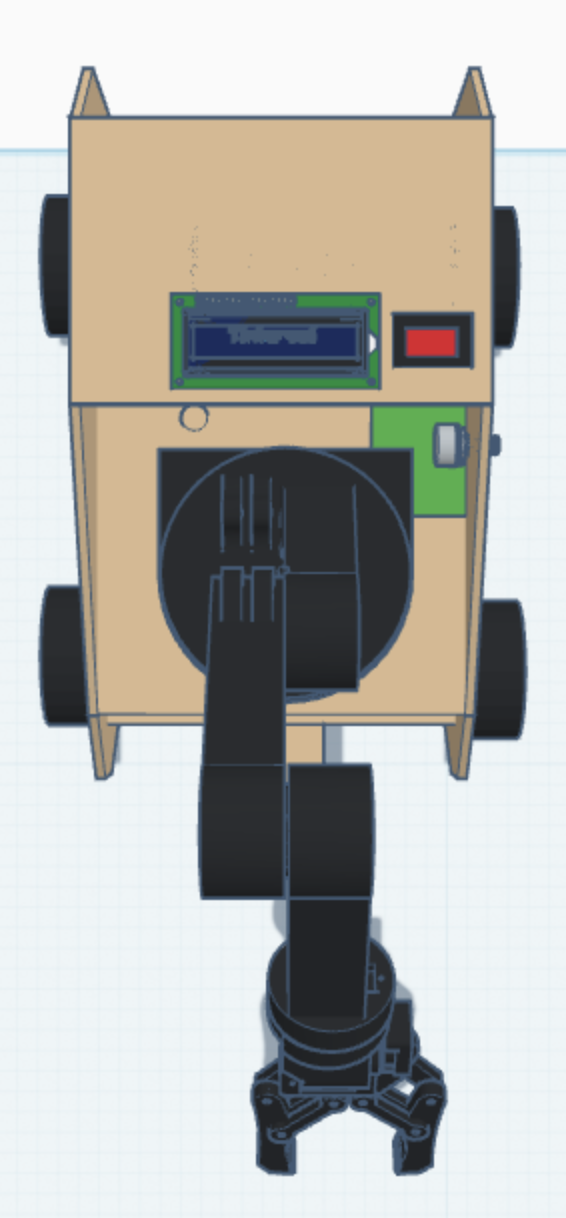
\includegraphics[height=4.5cm, keepaspectratio]{figure/robot_top.png}
        \caption{俯視圖}
        \label{fig:robot_top}
    \end{subfigure}
    \hfill
    \begin{subfigure}[b]{0.32\textwidth}
        \centering
        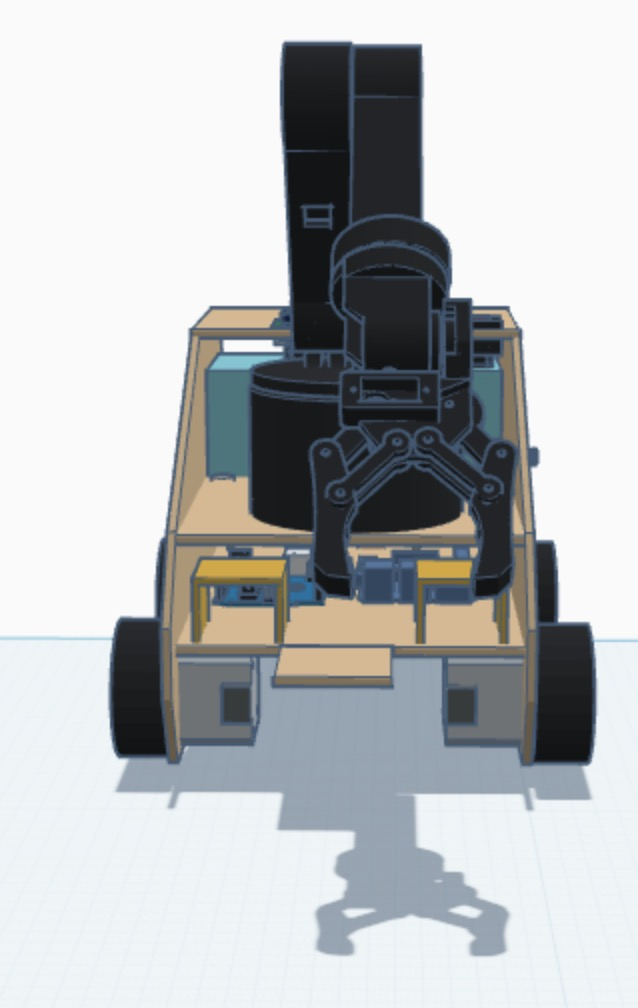
\includegraphics[height=4.5cm, keepaspectratio]{figure/robot_front.jpg}
        \caption{前視圖}
        \label{fig:robot_front}
    \end{subfigure}
    \hfill
    \begin{subfigure}[b]{0.32\textwidth}
        \centering
        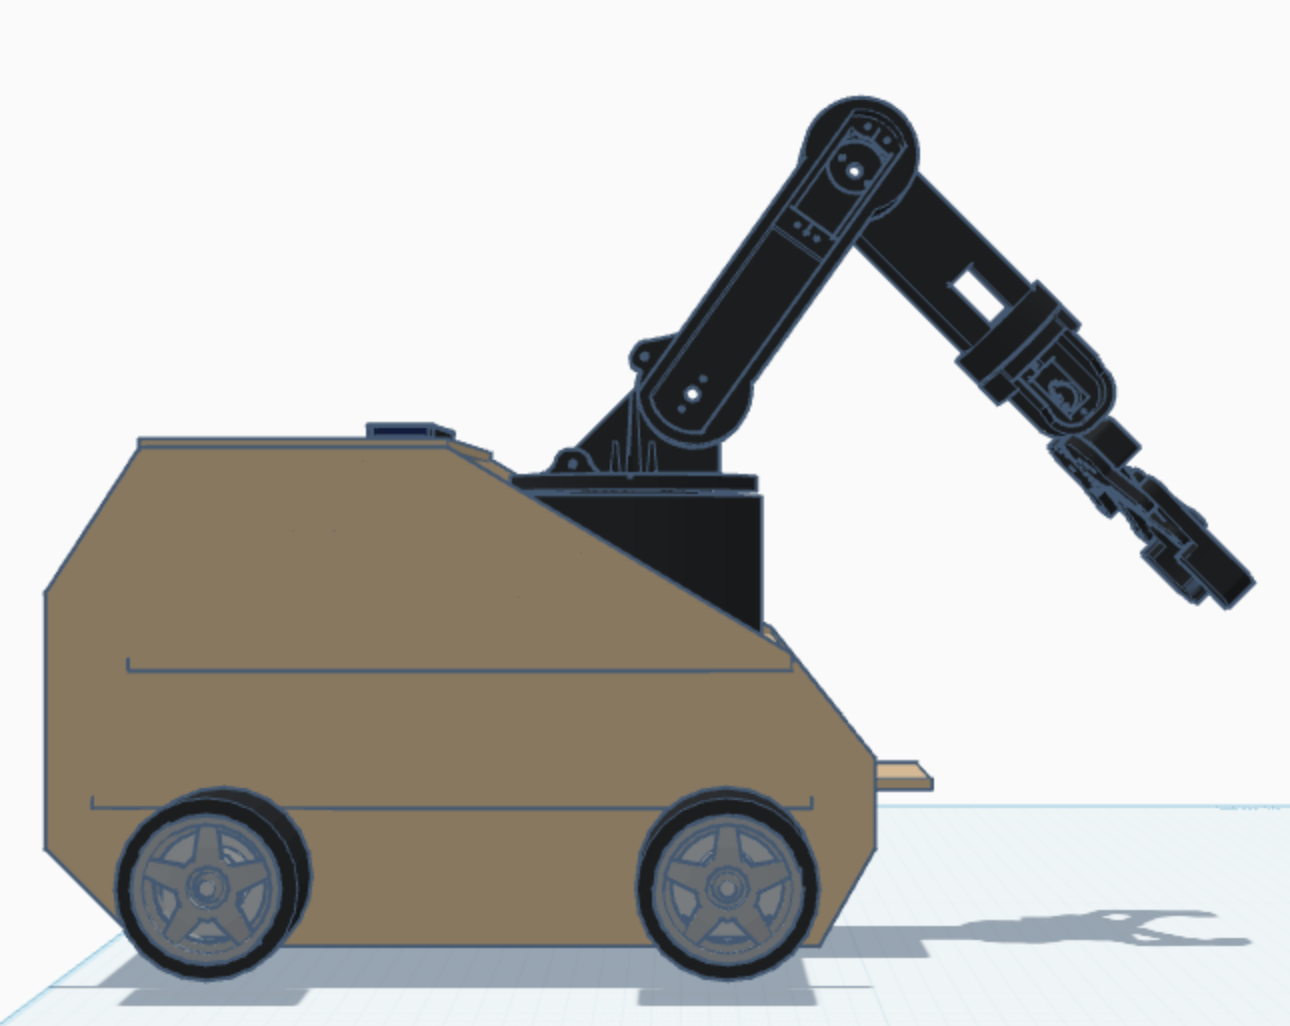
\includegraphics[width=\linewidth]{figure/robot_side.png}
        \caption{側視圖}
        \label{fig:robot_side}
    \end{subfigure}

    \vspace{0.3cm}

    \begin{subfigure}{0.7\textwidth}
        \centering
        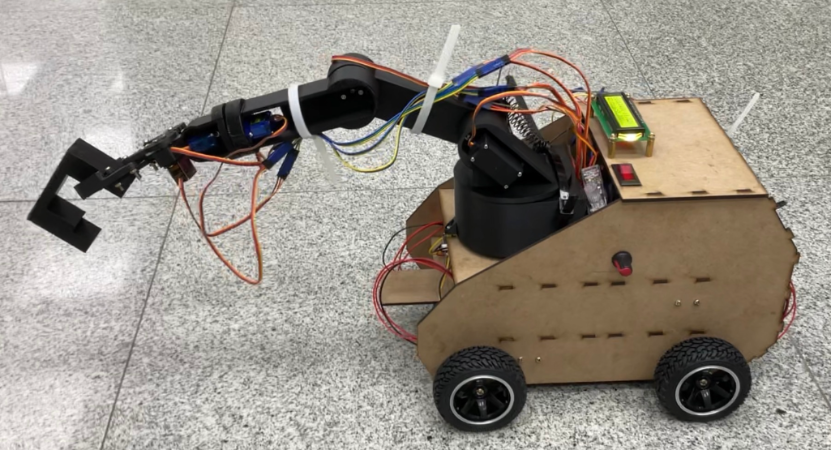
\includegraphics[width=\linewidth]{figure/robot_pickup.png}
        \caption{實際拾物圖}
        \label{fig:robot_pickup}
    \end{subfigure}

    \caption{抬底仔 (á)-Tidy UP 實際成品}
    \label{fig:actual_robot}
\end{figure}

\subsection{感測避障系統}

ESP32 搭配 HC-SR04 超聲波感測器與 SG90 伺服馬達，可對前方 180° 範圍進行掃描，即時顯示各角度之障礙物距離（圖 \ref{fig:detection}）。當障礙物距離低於安全閾值（8.4 cm）時，系統自動發出警示音提醒操作者，並於網頁介面更新雷達圖顯示最近物體方位。

\begin{figure}[H]
    \centering
    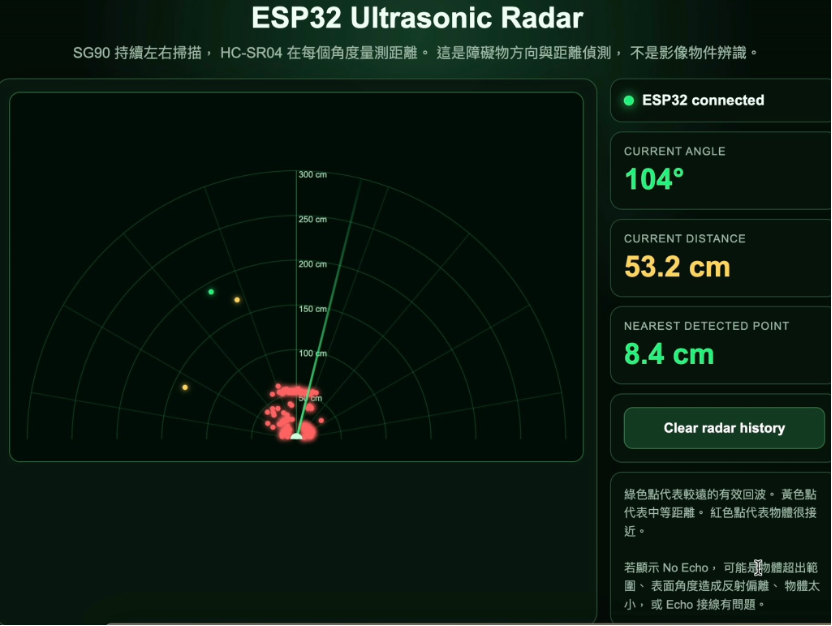
\includegraphics[width=0.65\linewidth]{figure/esp32_detection.png}
    \caption{ESP32 障礙物距離偵測介面（顯示當前角度 104°、距離 53.2 cm，最近安全點 8.4 cm）}
    \label{fig:detection}
\end{figure}

\subsection{遠端監控與控制系統}

Raspberry Pi 5 架設網頁伺服器，整合感測資訊顯示、底盤移動控制與機械手臂操作於單一介面（圖 \ref{fig:arm_control}）。操作者可透過任意裝置之瀏覽器在區域網路內連線，即時查看 ESP32 回傳之障礙物距離雷達圖，並以搖桿或按鈕控制底盤前後左右，以及機械手臂各關節角度與手爪的開合動作。

\begin{figure}[H]
    \centering
    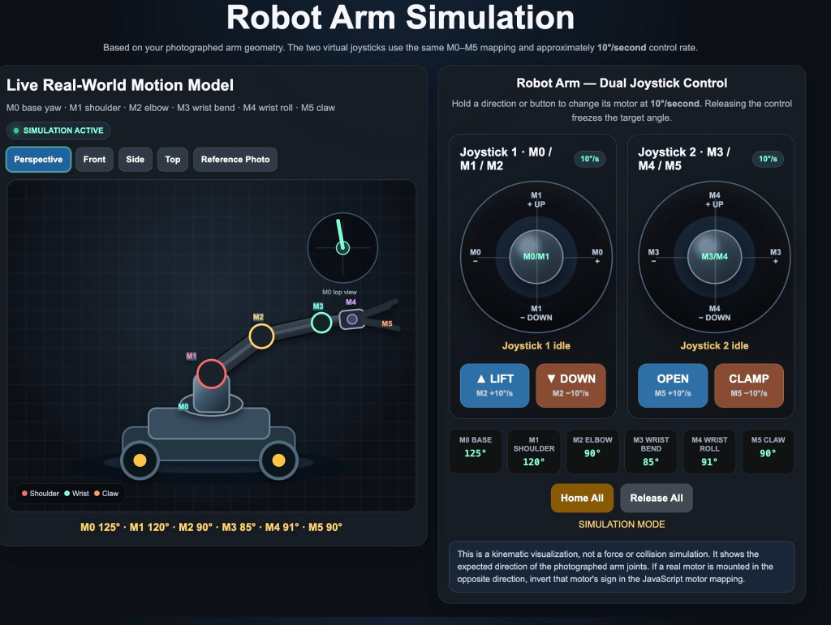
\includegraphics[width=0.75\linewidth]{figure/arm_control.png}
    \caption{機械手臂遠端控制網頁介面}
    \label{fig:arm_control}
\end{figure}

% ---------------------------------------------------------------
\section{成果討論}
% ---------------------------------------------------------------

\subsection{與初始目標之異同}

對照提案階段所設定之三項設計目標，分析實際成果如下：

\begin{enumerate}
  \setlength{\itemsep}{0.6em}

  \item \textbf{具備基本避障能力，在室內環境中安全移動：已達成。}

  ESP32 搭配 HC-SR04 能有效偵測 20--400 cm 範圍內的障礙物，於障礙物過近時發出警告，輔助操作者規避碰撞。然而，目前僅支援前向 180° 掃描，側向與後向仍有盲區，需操作者自行注意。

  \item \textbf{低成本、低能耗、低隱私疑慮，具備可擴充性：部分達成。}

  最終成本為 8,777 元，相較於偵測通報系統（兩年 16.3 萬）與居家照護（兩年 28.2 萬）仍具明顯優勢。系統採遠端操控而非攝影機監視，隱私疑慮低。然而實際成本較提案階段之估計（1,999 元）高出許多，主要原因為 Raspberry Pi 5 之導入與步進馬達系統之升級。Raspberry Pi 5 的模組化架構也為未來功能擴充（如加入攝影模組、YOLO 辨識）保留空間。

  \item \textbf{降低對長者主動整理環境的依賴：部分達成。}

  目前需由操作者（如家人或照護者）透過網頁介面遠端操控，而非完全自主運作，長者本身無法獨立使用。此與原規劃之全自主模式有所落差，但在「降低長者直接彎腰撿拾障礙物」的核心需求上已有所回應，透過遠端協作即可完成居家地面的整理工作。

\end{enumerate}

整體而言，本專案從原先規劃的「全自主 AI 辨識拾物」調整為「人機協同遠端遙控」，雖自主程度有所妥協，但實際可運作性更高，且核心功能（移動、避障、拾物、遠端操控）均已完整實現，系統架構也為往後的自主化升級保留了充分空間。

\subsection{與其他相關產品之比較}

市面上相關的居家輔助機器人（如 iRobot Roomba 等掃地機器人）主要聚焦於地面清潔，而非立體拾物，無法夾起拖鞋等具一定高度的散落物。Nissan 於 2018 年推出的 Self-Parking Slippers（Nissan, 2018）雖針對同樣的居家整齊議題設計，但其技術嵌入於特定拖鞋本身，成本高且易受翻面、位置偏移等不可控因素影響。

相較之下，抬底仔 (á)-Tidy UP 以通用拾物為設計目標，不依附於特定物品，並透過多軸機械手臂提供更高的夾取靈活性，在成本與通用性上具有明顯優勢，惟自主化程度與商業成熟產品相比仍有差距，尚需人工遠端操控輔助。

\subsection{未來展望}

\begin{enumerate}
  \setlength{\itemsep}{0.5em}
  \item \textbf{加入攝影模組與物件辨識：} 導入攝影模組，結合 YOLO 物件辨識模型（Redmon et al., 2016）使機器人能自動判斷物品種類、位置與適合的夾取方式（Wang et al., 2020），逐步降低對人工遠端操控的依賴，朝全自主目標推進。
  \item \textbf{改善機械結構：} 強化機械手臂的承重能力與手爪穩定度，並提升底盤在不同地面材質（地毯、磁磚）下的避障能力，提高不同大小與形狀物品的拾取成功率（Kumar et al., 2021）。
  \item \textbf{建立量化測試指標：} 包括定位誤差、拾取成功率、任務完成時間與續航能力，進一步進行實際居家環境與高齡使用者測試，為改進提供量化依據（Bardaro et al., 2022）。
\end{enumerate}

% ---------------------------------------------------------------
\section{Q\&A}
% ---------------------------------------------------------------

\textit{（本節記錄期末口頭報告時現場聽眾與評審之提問，以及本組之回覆。）}

\vspace{1em}
\noindent \textbf{Q1：}
目前車體底盤的輪子轉起來頓頓卡卡的，是什麼原因？
\vspace{0.5em}

\noindent \textbf{A1：}
因為車體底盤的輪子跟 LCD Palyer 共用同一個 Arduino UNO 版的關係，訊號會延遲導致卡頓。
在提問者的建議下，未來我們可以再裝一個 Arduino NANO 版移出來，既不佔空間，也可以解決訊號延遲問題。
\vspace{1.5em}

\noindent \textbf{Q2：}
超聲波感測器在測到很近的物體時會有誤差，這部分我們怎麼解決？
\vspace{0.5em}

\noindent \textbf{A2：}
我們目前還沒有做到量化拾取物品的距離與手臂要如何配合，因此我們後續會進行量化停車抓取的距離，來建立出最適合抓取物品的距離與動作。
\vspace{1.5em}

% ---------------------------------------------------------------
\section{課程心得}
% ---------------------------------------------------------------
\subsection*{張容爾}

修習這門課之前，我沒有任何正式的工程訓練背景。從車體結構設計、機械手臂的製作，到元件的配置與整合，每一個環節對我來說都是全新的挑戰。真正待在實驗室裡反覆調試、修正、再重來之後，我才慢慢體會到，原來工程設計的關鍵從來不是想到一個對的答案，而是在一次次行不通之後，停下來思考為什麼不行，並再重新校正方向與做法。最深刻的例子，是在發現手臂伺服馬達空轉問題，我們除了換成新的以外，也同時想知道為什麼會壞掉，因此就把伺服馬達拆開，才發現是齒輪鬆脫，我們小心翼翼把齒輪一組一組扳開，重新組回，也因此救回了好幾顆馬達。

我想特別謝謝我的兩位組員與幫助我們許多的助教群。盈翰從一開始就投入很多在系統架構與整合上，配電方式和元件的選用幾乎都是由他規劃；俊皓在發想階段就很積極，後續更承擔了大量的實作工作，沒有他們就不會有「抬底仔」。

我也要特別謝謝後期的俊皓，當專案到最後只剩我們兩個人時，他總是二話不說，利用課餘時間陪我一起進實驗室，debug 再怎麼不順利，他也還是很有耐心，從不因為又冒出新的問題而氣餒。雖然最後 demo 沒能呈現出我們原本期待的樣子，不但砍掉了不少功能，沒做出主動式避障，也沒有物件辨識，機械手臂甚至在 demo 前兩天還無法正常舉臂，當天又因為網路連線的問題，沒辦法把抬底仔和海報放在一起展示，但能夠做出一個功能完整、真的會動的成品，我還是覺得非常開心，很開心自己來到物理系修課，不但學到了很多工程實作的知識，也讓我對自己的興趣更了解了一些。


\subsection*{王俊皓}
其實這學期做這個實驗學習蠻多的，真的感受到每個隊員和助教的不同。盈翰的思考很快速且實作很強，總是可以brainstorm出很多想法，而且實行力很強。容爾在3D建模和各種機械組裝都非常擅長，機械手臂都是靠她組起來的，車子也是她畫出來並印出來的。然後也很感謝助教們總是在我們急需協助時，給我們很好的想法和建議，指引我們的活路。在這專案最有成就的地方就是看著這個車子長大，我看著它的線一個一個連起來，做了幾個實驗，把arduino板和電線燒斷，得知斷電的重要性。機械手臂沒電會舉不起來，沒裝彈簧協助，原來很重的手臂也舉不起來，原重量的扭力太大會把伺服馬達轉壞。即便我們把以上所有因素排除，伺服馬達的生產低良率還是把我們壓在地上打。容爾設計的手臂真的很好，但經過兩天的毒打，真的釐清很多問題，但即便把所有問題解決了，把事情看清了，在demo day還是無法看到在final project啟動第一週機械手臂健康的樣子，我們買的伺服馬達沒用就全壞了。但真的感謝隊員盈翰在一開始的系統整合與發想。和感謝容爾最後幾週的幫忙，沒日沒夜的趕工，最佳全勤獎，把專案扛在身上。感謝教授開蔗糖好課，讓我們能做這麼棒的專案訓練自己，並給予我那麼多雞湯；感謝助教幫忙，給我們超多建議指引我們；最後感謝最重要的隊友，讓我能夠參與這個專案，學習到很多東西。在此之前，我是對電機工程完全失去興趣的學生，因為一些沒那麼明智的抉擇，走了些歪路，把自己的興趣磨滅掉，但我在這堂課，我找回了些學習熱忱，其實更重要的是，我看到了隊友在專案的責任感和付出，consistenty和commitment，讓我學到了在科學領域最重要的事情。雖然我不是那麼高效的人，但在這個專案，我有找到更多讓自己成長的方法。感謝大家愛這堂課

\vspace{4em}

\clearpage
\section*{參考文獻}
國家衛生研究院高齡醫學暨健康福祉研究中心。（n.d.）。僅高齡人口居住宅數變化。臺灣高齡健康與長照服務年報。\url{https://ageing.nhri.edu.tw/annual_report/tCSMjW1F27USj12UCMW99}

衛生福利部。（2019 年 9 月 24 日）。每 6 人就有 1 位老人曾跌倒 國健署傳授防跌妙招。\url{https://www.mohw.gov.tw/cp-4253-49428-1.html}

衛生福利部統計處。（2021 年 7 月 2 日）。107 年國人死因統計結果。\url{https://dep.mohw.gov.tw/dos/lp-5069-113-xCat-y107.html}

衛生福利部國民健康署。（n.d.）。老人跌倒常見的危險因子有那些？\url{https://www.hpa.gov.tw/Pages/Detail.aspx?nodeid=807&pid=4327}

Cook, D. J., \& Das, S. K. (Eds.). (2004). \textit{Smart environments: Technologies, protocols, and applications}. Wiley. \url{https://onlinelibrary.wiley.com/doi/book/10.1002/047168659X}

Nissan. (2018, January 25). \textit{Hotel guests get a kick out of Nissan's self-parking slippers}. \url{https://global.nissannews.com/releases/180125-01-e?lang=en}

Pynoos, J., Steinman, B. A., \& Nguyen, A. Q. D. (2010). Environmental assessment and modification as fall-prevention strategies for older adults. \textit{Clinics in Geriatric Medicine, 26}(4), 633--644. \url{https://pubmed.ncbi.nlm.nih.gov/20934614/}

TIME. (2025, July 23). \textit{Why so many seniors can't afford long-term care}. \url{https://time.com/7304510/seniors-long-term-care-costs/}

Wang, X., Ellul, J., \& Azzopardi, G. (2020). Elderly fall detection systems: A literature survey. \textit{Frontiers in Robotics and AI, 7}, 71. \url{https://pmc.ncbi.nlm.nih.gov/articles/PMC7805655/}

Bardaro, G., Antonini, A., \& Motta, E. (2022). Robots for elderly care in the home: A landscape analysis and co-design toolkit. \textit{International Journal of Social Robotics, 14}(3), 657--681. \url{https://link.springer.com/article/10.1007/s12369-021-00816-3}

Kumar, A., et al. (2021). \textit{Autonomous bot with ML-based reactive navigation for indoor environment}. arXiv. \url{https://arxiv.org/pdf/2111.12542}

Redmon, J., Divvala, S., Girshick, R., \& Farhadi, A. (2016). You only look once: Unified, real-time object detection. In \textit{Proceedings of the IEEE conference on computer vision and pattern recognition} (pp. 779--788). \url{https://arxiv.org/abs/1506.02640}

CGTrader. (n.d.). \textit{Arduino obstacle avoiding robot car} [3D model]. \url{https://www.cgtrader.com/free-3d-print-models/hobby-diy/electronics/arduino-obstacle-avoiding-robot-car}

Instructables. (n.d.-a). \textit{I made an excavator with a working arm to scoop things as well as working motors that make it drive and turn}. \url{https://www.instructables.com/I-Made-an-Excavator-With-a-Working-Arm-to-Scoop-Th/}

Instructables. (n.d.-b). \textit{TBB tractor robot with tractor scoop accessory}. \url{https://www.instructables.com/TBB-Tractor-Robot-With-Tractor-Scoop-Accessory/}

\end{document}
